% 第二章:导数与微分
\chapter{导数与微分}
\section{导数的定义}
\begin{example}{}{}
    已知$x,y>0$,且$x^2+9y^2=12$,则$\dfrac{x+2}{y+1}-3x$的最小值为\underline{\hspace{2cm}}.
\end{example}
\begin{solution}

\end{solution}
\begin{example}{}{}
    (单选)数列$a_{n}$各项为正整数且递增,$a_{n+2}=C_{a_{n+1}}^{a_{n}}$,则(~~~~~)

    \begin{tabular}{@{}ll@{}}
        A.$a_n<a_{n-1}+1$&B.$a_1,a_2,a_3$可能成等比数列\\
        C.$a_3a_4<a_5$&D.$a_3,a_4,a_5$可能成等比数列
    \end{tabular}
\end{example}
\begin{solution}
由于$a_n$递增,则A显然错误;下面考虑选项BD:
\[
    a_na_{n+2} = a_nC_{a_{n+1}}^{a_{n}}=a_{n+1}C_{a_{n+1}-1}^{a_{n}-1}=a_{n+1}^2\\\Rightarrow a_{n+1}=C_{a_{n+1}-1}^{a_{n}-1}
\]

当$a_n=1$时,代入表达式得到$a_{n+1}=C_{a_{n+1}-1}^{0}=1=a_n$,与数列递增矛盾;

当$a_n=2$时,代入表达式得到$a_{n+1}=C_{a_{n+1}-1}^{1}=a_{n+1}-1<a_{n+1}$,矛盾;

当$a_n>2$时,易得$a_{n+1}-1>2$,代入表达式得到
\[a_{n+1}=C_{a_{n+1}-1}^{a_{n}-1}\ge C_{a_{n+1}-1}^{2}=\dfrac{(a_{n+1}-1)(a_{n+1}-2)}{2}\]

解方程发现无整数解,而且由于$C_{a_{n+1}-1}^{1}=a_{n+1}-1$是小于$a_{n+1}$的最大整数,且有

\[C_{a_{n+1}-1}^{1}<C_{a_{n+1}-1}^{2},~~C_{a_{n+1}-1}^{2}\ne a_{n+1}\]

只可能是$C_{a_{n+1}-1}^{2}> a_{n+1}$.

雪上加霜的是,$C_{a_{n+1}-1}^{2}$和$C_{a_{n+1}-1}^{1}$中间没有数可以等于$C_{a_{n+1}-1}^{m}$,所以BD错误;

考虑C,易得$a_1\ne1,a_2\ge 4,a_3\ge6,a_4=C_{a_3}^{a_2}>2a_3+1$,由
\[a_5=C_{a_4}^{a_3}>a_3a_4 \Rightarrow a_3^2<C_{a_{4}-1}^{a_{3}-1}<C_{2a_3}^{a_3-1}\]

转化为$a_3^3+a_3<C_{2a_3}^{a_3}$这是显然成立的,故本题目选C
\end{solution}
\begin{example}{}{}
    已知$\triangle{ABC}$中,$A=3B=9C$,则$\cos A\cos B+\cos B\cos C+\cos C\cos A=$\underline{\hspace{1cm}}.
\end{example}
\begin{solution}
解得$A=\dfrac{9\pi}{13},B=\dfrac{3\pi}{13},C=\dfrac{\pi}{13}$考虑积化和差:
\begin{align*}
&\cos A\cos B+\cos B\cos C+\cos C\cos A\\
&=\dfrac12(\cos(A+B)+\cos(A-B)+\cos(B+C)+\cos(B-C)+\cos(A+C)+\cos(A+C))\\
&=\dfrac12(\cos\dfrac{12\pi}{13}+\cos\dfrac{6\pi}{13}+\cos\dfrac{4\pi}{13}+\cos\dfrac{2\pi}{13}+\cos\dfrac{10\pi}{13}+\cos\dfrac{8\pi}{13})\\
&=\dfrac{1}{2\sin\dfrac{\pi}{13}}\sin\dfrac{\pi}{13}(\cos\dfrac{2\pi}{13}+\cos\dfrac{4\pi}{13}+\cos\dfrac{6\pi}{13}+\cos\dfrac{8\pi}{13}+\cos\dfrac{10\pi}{13}+\cos\dfrac{12\pi}{13})\\
&=\dfrac{1}{4\sin\dfrac{\pi}{13}}(\sin\dfrac{\pi}{13}-\sin\dfrac{3\pi}{13}+\sin\dfrac{3\pi}{13}-\sin\dfrac{5\pi}{13}+\sin\dfrac{5\pi}{13}-\sin\dfrac{7\pi}{13}\\
&~~~~~~~~~~~~~~~~+\sin\dfrac{7\pi}{13}-\sin\dfrac{9\pi}{13}+\sin\dfrac{9\pi}{13}-\sin\dfrac{11\pi}{13}+\sin\dfrac{11\pi}{13}-\sin\dfrac{13\pi}{13})\\
&=-\dfrac14
\end{align*}
\end{solution}
\begin{theorem}{阿贝尔求和}{}
    设$B_n$是数列$b_n$的前$n$项和,当$n\ge 2$时,有:\vspace{-5pt}\[
    \sum_{i=1}^na_ib_i=a_nB_n-\sum_{i=1}^{n-1}(a_{i+1}-a_i)B_n\]
\end{theorem}
\begin{myproof}
    当$n\ge 2$时,有
    \begin{align*}
        \sum_{i=1}^na_ib_i=&a_1b_1+\sum_{i=2}^{n}a_i(B_i-B_{i-1})\\
        =&a_1b_1+\sum_{i=2}^{n}a_iB_i-\sum_{i=2}^{n}a_iB_{i-1}\\
        =&\sum_{i=1}^{n}a_iB_i-\sum_{i=1}^{n-1}a_{i+1}B_i\\
        =&a_nB_n-\sum_{i=1}^{n-1}(a_{i+1}-a_i)B_n
    \end{align*}
\end{myproof}
\begin{example}{(来自Fiddie)}{}
    设数列$\{a_n\}$的各项均为实数,且当$n\ge 2$时,$a_{n+1}+a_{n-1}=|a_n|$.证明:

    (1)存在大于$1$的正整数$m$使得$a_m\le 0$

    (2)存在正整数$m$使得$a_m\le 0,~a_{m+1}\le 0$

    (3)$a_n=a_{n+9}$ 
\end{example}
\begin{solution}
    (1)当$n\ge 2$时,由\[
    \begin{cases}a_{n+1}+a_{n-1}=|a_n|\\a_{n+2}+a_{n}=|a_{n+1}|\end{cases}\Rightarrow a_{n+2}+a_{n+1}+a_n+a_{n-1}=|a_n|+|a_{n+1}|
    \]\[
    \Rightarrow a_{n+2}+a_{n-1}=|a_n|-a_n+|a_{n+1}|-a_{n+1}\ge 0
    \]
    若$n\ge 2$时$a_n>0$,上式化为$a_{n+2}+a_{n-1}=0$,矛盾,故存在大于$1$的正整数$m$使得$a_m\le 0$
 
    \noindent(2)已证存在大于$1$的整数$m$使得$a_m\le 0$,现假设不存在正整数$k$使得$a_k\le 0,~a_{k+1}\le 0$,则不妨设$a_m$为首个小于等于$0$的项,由假设得$a_1,a_2,...a_{m-1}>0,a_m\le 0, a_{m+1}>0$,可以通过不断消元推出矛盾:\vspace{-10pt}
    \begin{align*}
    a_{m+1}+a_{m-1}=|a_m|&=-a_m\Rightarrow a_{m+1}=-a_m-a_{m-1}\\
    a_{m+2}+a_m=|a_{m+1}|&=a_{m+1}\Rightarrow a_{m+2}=a_{m+1}-a_m>0+0=0\\
    a_{m+3}+a_{m+1}=|a_{m+2}|&=a_{m+2}\Rightarrow a_{m+3}=a_{m+2}-a_{m+1}=a_{m+1}-a_m-a_{m+1}=-a_m\geq 0\\
    a_{m+4}+a_{m+2}=|a_{m+3}|&=-a_{m}\Rightarrow a_{m+4}=-a_{m}-a_{m+2}=-a_{m+1}<0\\
    a_{m+5}+a_{m+3}=|a_{m+4}|&=a_{m+1}\Rightarrow a_{m+5}=a_{m+1}-a_{m+3}=a_m+a_{m+1}=-a_{m-1}<0
    \end{align*}
    由$a_{m+4}<0,a_{m+5}<0$知矛盾,故存在正整数$k$使得$a_k\le 0,~a_{k+1}\le 0$.

\noindent(3)抓住上面第二小问的提示就可以得到:
    \vspace{-5pt}\begin{align*}
    a_{m+6}+a_{m+4}=|a_{m+5}|&=a_{m-1}\Rightarrow a_{m+6}=a_{m-1}-a_{m+4}=a_{m-1}+a_{m+1}=-a_m\\
    a_{m+7}+a_{m+5}=|a_{m+6}|&=-a_{m}\Rightarrow a_{m+7}=-a_{m}-a_{m+5}=a_{m-1}-a_m\\
    a_{m+8}+a_{m+6}=|a_{m+7}|&=a_{m-1}-a_m\Rightarrow a_{m+8}=a_{m-1}-a_m-a_{m+6}=a_{m-1}\\
    a_{m+9}+a_{m+7}=|a_{m+8}|&=a_{m-1}\Rightarrow a_{m+9}=a_{m-1}-a_{m+7}=a_{m-1}-a_{m-1}+a_{m}=a_m
    \end{align*}\vspace{-15pt}
    所以设$T=9$,有\[\begin{cases}a_{m}=a_{m+nT},n\in N\\a_{m-1}=a_{m-1+nT},n\in N\end{cases}\]
    然后由于\[a_{m-2+nT}=|a_{m-1+nT}|-a_{m+nT}=|a_{m-1}|-a_{m}=a_{m-2}\]以此类推,则有\[
    a_k=a_{k+nT},k\in N_+,k\leq m\]取合适的$m$使得$m$大于$T$,则数列$\{a_n\}$为周期数列,其中一个周期为9
\end{solution}
\begin{example}{(南通9调14题)}{}
    已知$x,y$满足$(\sqrt{x^2+1}-x)(\sqrt{y^2+4}-y)=2$,则$4^{x}+2^{y-1}$的最小值为\underline{\hspace{1cm}}.
\end{example}
\begin{solution}
    套路题,先换元:\[
    \begin{cases}
        m=\sqrt{x^2+1}-x\Rightarrow x=\dfrac{1}{2m}-\dfrac{2}{m}\\[8pt]
        n=\sqrt{y^2+4}-y\Rightarrow y=\dfrac{2}{n}-\dfrac{n}{2}\end{cases}
    \]
    再代入$mn=2\Rightarrow n=\dfrac{2}{m}$:
    \[y=\dfrac{2}{n}-\dfrac{n}{2}=m-\dfrac{1}{m}\Rightarrow y=-2x\]
    所以:\[4^{x}+2^{y-1}=4^{x}+\dfrac{1}{2\times 4^x}\geq 2\sqrt{\dfrac{1}{2}}=\sqrt2\]当$x=\frac14$时取得等号
\end{solution}
\newpage
\begin{example}{(深圳中学2025届二轮一阶)}{}
    \noindent$\triangle{ABC}$中,若
    \[\begin{cases}\overrightarrow{AD}=\dfrac{\lambda}{\lambda+1}\overrightarrow{AC}\\
        \overrightarrow{AE}=\dfrac{\mu}{\mu+1}\overrightarrow{AB}\end{cases}\]
    \noindent 则连接$BD,CE$得到交点$Q$,任取$\triangle{ABC}$所在平面内某一点$P$,那么有:\[
    PQ^2=\dfrac{PA^2+\mu PB^2+\lambda PC^2}{1+\lambda+\mu}-\dfrac{\lambda\mu BC^2+\lambda AC^2+\mu AB^2}{\left(1+\lambda+\mu\right)^2}
    \]
\end{example}
\begin{solution}
      设\[
      \begin{cases}\overrightarrow{AQ}=x\overrightarrow{AD}+(1-x)\overrightarrow{AB}=x\dfrac{\lambda}{1+\lambda}\overrightarrow{AC}+(1-x)\overrightarrow{AB}\\[10pt]
      \overrightarrow{AQ}=y\overrightarrow{AE}+(1-y)\overrightarrow{AC}=y\dfrac{\mu}{1+\mu}\overrightarrow{AB}+(1-y)\overrightarrow{AC}\end{cases}\Rightarrow \begin{cases}x=\dfrac{\lambda+1}{1+\lambda+\mu}\\[8pt]y=\dfrac{\mu+1}{1+\lambda+\mu}\end{cases}
      \]
      化为形如$x\overrightarrow{QA}+y\overrightarrow{QB}+z\overrightarrow{QC}=0$的方程:
      \begin{align*}
          \Rightarrow \overrightarrow{AQ}&=\dfrac{\lambda}{1+\lambda+\mu}\overrightarrow{AC}+\dfrac{\mu}{1+\lambda+\mu}\overrightarrow{AB}\\
          &=\dfrac{\lambda}{1+\lambda+\mu}(\overrightarrow{AQ}+\overrightarrow{QC})+\dfrac{\mu}{1+\lambda+\mu}(\overrightarrow{AQ}+\overrightarrow{QB})\\
          &=\dfrac{\lambda+\mu}{1+\lambda+\mu}\overrightarrow{AQ}+\dfrac{\lambda}{1+\lambda+\mu}\overrightarrow{QC}+\dfrac{\mu}{1+\lambda+\mu}\overrightarrow{QB}\\
          \Rightarrow \overrightarrow{QA}&+\lambda\overrightarrow{QC}+\mu\overrightarrow{QB}=\vec{0}\\
          \Rightarrow \overrightarrow{PA}&-\overrightarrow{PQ}+\lambda(\overrightarrow{PC}-\overrightarrow{PQ})+\mu(\overrightarrow{PB}-\overrightarrow{PQ})=\vec{0}\\
          \Rightarrow \overrightarrow{PA}&+\lambda\overrightarrow{PC}+\mu\overrightarrow{PB}=(1+\lambda+\mu)\overrightarrow{PQ}
      \end{align*}
    平方得:\[
PA^2+\lambda^2PC^2+\mu^2PB^2+2\lambda\overrightarrow{PA}\cdot\overrightarrow{PC}+2\mu\overrightarrow{PA}\cdot\overrightarrow{PB}+2\lambda\mu\overrightarrow{PC}\cdot\overrightarrow{PB}=(1+\lambda+\mu)^2PQ^2\]分别
代入\[\begin{cases}2\lambda\overrightarrow{PA}\cdot\overrightarrow{PC}=\lambda\bigg(PA^2+PC^2-(\overrightarrow{PA}-\overrightarrow{PC})\bigg)^2=\lambda(PA^2+PC^2-AC^2)\\
    2\mu\overrightarrow{PA}\cdot\overrightarrow{PB}=\mu\bigg(PA^2+PB^2-(\overrightarrow{PA}-\overrightarrow{PB})\bigg)^2=\mu(PA^2+PB^2-AB^2)\\
    2\lambda\mu\overrightarrow{PC}\cdot\overrightarrow{PB}=\lambda\mu\bigg(PC^2+PB^2-(\overrightarrow{PC}-\overrightarrow{PB})\bigg)^2=\lambda\mu(PC^2+PB^2-BC^2)
\end{cases}\]
    变形即可得到:\[
    PQ^2=\dfrac{PA^2+\mu PB^2+\lambda PC^2}{1+\lambda+\mu}-\dfrac{\lambda\mu BC^2+\lambda AC^2+\mu AB^2}{\left(1+\lambda+\mu\right)^2}\]
\end{solution}
因此有结论:
\begin{conclusion}{结论}{}
    \noindent 平面内给定$\triangle{ABC}$,若点$Q$满足\vspace{-10pt}
    \[\overrightarrow{QA}+\lambda\overrightarrow{QC}+\mu\overrightarrow{QB}=\vec{0}\vspace{-10pt}\]则任取$\triangle{ABC}$所在平面内某一点$P$,有\[PQ^2=\dfrac{PA^2+\mu PB^2+\lambda PC^2}{1+\lambda+\mu}-\dfrac{\lambda\mu BC^2+\lambda AC^2+\mu AB^2}{\left(1+\lambda+\mu\right)^2}\]
\end{conclusion}
\begin{example}{三角形外心坐标}{}
    已知平面直角坐标系$xOy$中有一个$\triangle{ABC}$,则其外心的坐标为\[
    \left(\dfrac{\begin{vmatrix}
    OA^2 & y_A & 1\\
    OB^2 & y_B & 1\\
    OC^2 & y_C & 1\\
\end{vmatrix}}{2\begin{vmatrix}
    x_A & y_A & 1\\
    x_B & y_B & 1\\
    x_C & y_C & 1\\
\end{vmatrix}},\dfrac{\begin{vmatrix}
    x_A & OA^2 & 1\\
    x_B & OB^2 & 1\\
    x_C & OC^2 & 1\\
\end{vmatrix}}{2\begin{vmatrix}
    x_A & y_A & 1\\
    x_B & y_B & 1\\
    x_C & y_C & 1\\
\end{vmatrix}}\right)
\]\end{example}
\begin{solution}

\end{solution}
\begin{example}{三角形垂心坐标}{}
    已知平面直角坐标系$xOy$中有一个$\triangle{ABC}$,则其垂心的坐标为\[
    \left(\dfrac{\begin{vmatrix}
    x_Bx_C+y_By_C & y_A & 1\\
    x_Ax_C+y_Ay_C & y_B & 1\\
    x_Ax_B+y_Ay_B & y_C & 1\\
    \end{vmatrix}}{-\begin{vmatrix}
    x_A & y_A & 1\\
    x_B & y_B & 1\\
    x_C & y_C & 1\\
    \end{vmatrix}},\dfrac{\begin{vmatrix}
    x_A & x_Bx_C+y_By_C & 1\\
    x_B & x_Ax_C+y_Ay_C & 1\\
    x_C & x_Ax_B+y_Ay_B & 1\\
    \end{vmatrix}}{-\begin{vmatrix}
    x_A & y_A & 1\\
    x_B & y_B & 1\\
    x_C & y_C & 1\\
    \end{vmatrix}}\right)\]
\end{example}
\begin{example}{容斥原理练习}{}
    某学校举办比赛,有$20$个参赛名额,现在分给$4$个不同的班,保证至少有一个班的名额为$4$个,且每一个班都有名额,则共有\underline{\hspace{1cm}}种分法。
\end{example}
\begin{solution}
    设四个班的名额为$x_1,x_2,x_3,x_4\in N_+$,则分法数就是集合$A_i=\{(x_1,x_2,x_3,x_4)|x_i=4,x_1+x_2+x_3+x_4=20\}$的元素个数,又因为
    \begin{align*}|A_{1}|&=\{(x_{1},x_{3},x_{4})\mid x_{2}+x_{3}+x_{4}=16,x_{2},x_{3},x_{4}>0\}=C_{15}^{2}\\|A_{1}\cap A_{2}|&=\{(x_{3},x_{4})\mid x_{3}+x_{4}=12,x_{3},x_{4}>0\}=C_{11}^{1}\\|A_{1}\cap A_{2}\cap A_{3}|&=1\\
    |A_1\cup A_2\cup A_3\cup A_4|&=C_4^1|A_1|-C_4^2|A_1\cap A_2|+C_4^3|A_1\cap A_2\cap A_3|\\
        &=C_4^1C_{15}^2-C_4^2+C_4^3C_{11}^1=358\end{align*}
\end{solution}
\newpage
\begin{example}{求和}{}
    计算$\displaystyle \sum_{i=0}^{n-1}(-1)^{i}C_{n-1}^{i}(i+1)^k$,其中$k<n-1,k\in N_+$
\end{example}
\begin{solution}
    定义函数并对其求$k$阶导数:\begin{align*}f(x)=&\displaystyle\sum_{i=0}^{n-1}(-1)^{i}C_{n-1}^{i}x^{i+1}
        =\displaystyle x\sum_{i=0}^{n-1}(-x)^{i}C_{n-1}^{i}\\
        =&\displaystyle x(1-x)^{n-1}
        =(x-1+1)(1-x)^{n-1}
        =(1-x)^{n-1}-(1-x)^n\\
    \Rightarrow f(1)=&\displaystyle\sum_{i=0}^{n-1}(-1)^{i}C_{n-1}^{i}=0\\
     f^{(k)}(x)=&\displaystyle\sum_{i=0}^{n-1}(-1)^{i}C_{n-1}^{i}A_{i+1}^{k}x^{i+1-k}\Rightarrow
     f^{(k)}(1)=\displaystyle\sum_{i=0}^{n-1}(-1)^{i}C_{n-1}^{i}A_{i+1}^{k}
    \end{align*}
    现已很接近原式,问题在于沟通$A_{i+1}^{k}$和${(i+1)}^{k}$,我们假想这样一个情境:有$k$个不同的球等待放进$i+1$个不同的盒子里面,放置过程中允许空盒的存在,所以放法是${(i+1)}^{k}$,然后我们换一种方式,考虑分为恰好有$0,1,2,3,4,...,k$个非空盒子的情况,那么求和就是\[\sum_{r=0}^kS(k,r)r!C_{i+1}^r=\sum_{r=0}^kS(k,r)A_{i+1}^r\]
    其中$S(k,r)$表示$k$个有标号的球放到r个同样的盒子里面的方法数,$C_{i+1}^r$表示从$i+1$个不同的盒子无序地挑出$r$个盒子来放球,再对其进行全排列使得挑出来的$r$个盒子有编号,则:\[(i+1)^{k}=\sum_{r=0}^kS(k,r)A_{i+1}^r
    \]
    那么代入到$\displaystyle \sum_{i=0}^{n-1}(-1)^{i}C_{n-1}^{i}(i+1)^k$中就有:\begin{align*}
    \sum_{i=0}^{n-1}(-1)^{i}C_{n-1}^{i}(i+1)^k=&\sum_{i=0}^{n-1}\bigg((-1)^{i}C_{n-1}^{i}\bigg(\sum_{r=0}^kS(k,r)A_{i+1}^r\bigg)\bigg)\\=&\sum_{i=0}^{n-1}\sum_{r=0}^kS(k,r)A_{i+1}^r(-1)^{i}C_{n-1}^{i}\\=&\sum_{r=0}^k\sum_{i=0}^{n-1}S(k,r)A_{i+1}^r(-1)^{i}C_{n-1}^{i}=\sum_{r=0}^kS(k,r)f^{(r)}(1)
    \end{align*}
    对$(1-x)^{n-1}-(1-x)^n$求导易得$f(x)$只有第$n-1$和$n$阶导数在$x=1$处的值不是$0$,即:\[\sum_{i=0}^{n-1}(-1)^{i}C_{n-1}^{i}(i+1)^k=0
    \]
\end{solution}
% 图片插入示例(注释掉,避免报错)
% \begin{figure}[htbp]
%     \centering
%     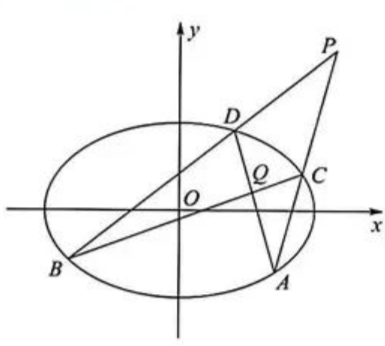
\includegraphics[width=0.6\textwidth]{flg/example.png}
%     \caption{导数的几何意义}
%     \label{fig:derivative}
% \end{figure}